\subsection*{\hypertarget{monster}{Monstruos}}
"Cada día que pasa, el mundo encuentra nuevas y emocionantes formas de matar a un hombre".\\
\indent -- Balthier
\vspace*{0.3cm}
\begin{center} 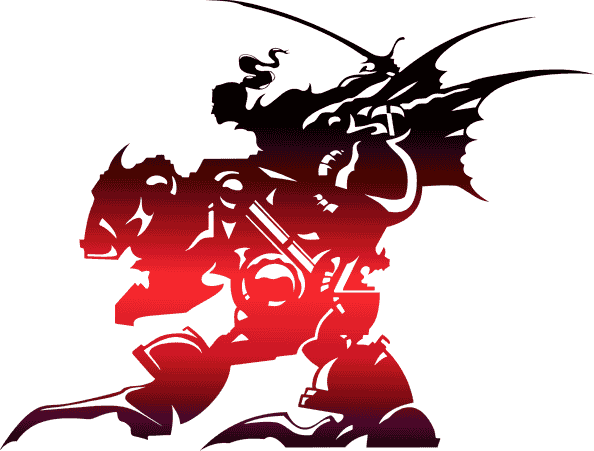
\includegraphics[width=\columnwidth]{./art/images/ff6.png} \end{center}
\vspace*{0.3cm}
\addcontentsline{toc}{subsection}{Monstruos}%
Los monstruos son seres salvajes similares a los animales que habitan lugares no civilizados del mundo. Normalmente tienen un hábitat natural en el que intentan sobrevivir, así que al cruzarse con el grupo se sentirán amenazados y atacarán. Los distintos tipos de monstruos suelen aliarse para atacar al grupo, aunque en algunas ocasiones puede que no sea así. El grupo también puede enfrentarse a monstruos más poderosos e inteligentes cuando los objetivos son más complejos. Los monstruos suelen ser parte o causa de los conflictos, por lo tanto, el grupo se enfrentará a ellos con bastante frecuencia. \subsubsection*{Creación de monstruos}
Generalmente, el mundo que crees incluirá diferentes tipos de monstruos que el grupo tendrá que enfrentar durante su aventura. Puedes utilizar las siguientes directivas para crear tus propios monstruos.

\begin{description}[leftmargin=*]

\item[\color{accent} Contexto:] Al crear un monstruo, es importante considerar en qué circunstancias se enfrentarán al grupo. Debido a las normas de combate, el lado que tenga más integrantes tendrá más ventajas ya que pueden tomar más acciones por ronda. Por lo tanto, los enemigos potentes pero superados en número a menudo tendrán que compensarlo con atributos y habilidades mucho más potentes. Además, debes asegurarte de ajustar la dificultad de los monstruos teniendo en cuenta la experiencia del grupo con el juego. \item[\color{accent} Atributos:] Los atributos de los personajes después del Nivel 1 se distribuyen de la siguiente manera, que puedes utilizar como regla general: para cada Subida de nivel, un personaje obtiene 5 puntos de atributos, donde un punto equivale a 5 PV/PM o 1 FUE/DEF/MAG/RES.
\pagebreak
La AGI en general debería ser de entre 1 y 5, pero los monstruos con baja AGI deberían compensar en otros aspectos. A diferencia de los personajes, los monstruos también pueden variar significativamente de tamaño, lo que puede tener un gran efecto en la batalla. Aunque los monstruos no utilizan armas y armaduras tradicionales, tienen partes equivalentes integradas en sus cuerpos que se ajustan a las mismas reglas. \item[\color{accent} Habilidades:] Los monstruos también pueden utilizar Magia y Técnicas, así como Habilidades Pasivas y de Reacción. Sin embargo, intenta mantener el número de habilidades de los monstruos al mínimo para tomar decisiones rápidas durante el combate. No obstante, puedes darles a los monstruos habilidades únicas y exóticas para hacerlos más interesantes. \item[\color{accent} Resistencias y Debilidades:] Puedes hacer que la estrategia de ataque contra tus monstruos sea más compleja utilizando resistencias y debilidades a tipos de daño específicos. Normalmente, los monstruos de nivel bajo tienden a tener más debilidades, mientras que los monstruos más poderosos a menudo resisten ciertos tipos de daño. A diferencia de los personajes, los monstruos también pueden ser naturalmente inmunes a diversos estados alterados y a algunos tipos de daño. Durante el combate, puedes dar pistas sutiles a los jugadores sobre las fortalezas y debilidades de un enemigo cuando narran las acciones de combate y sus efectos. \item[\color{accent} Humanoides:] Si quieres crear un enemigo humanoide, sigue las reglas de personaje en la \hyperlink{char}{Sección Personajes}. Dependiendo de la importancia del enemigo, puedes obviar detalles que consideres innecesarios. Crear una hoja de personaje completa vale la pena solo para los antagonistas principales. También ten en cuenta que los enemigos humanoides pueden utilizar y mejorar su equipo y sus objetos al igual que los personajes de los jugadores. 
	
\end{description}

\subsubsection*{Ejemplos}
A continuación verás algunos ejemplos de monstruos que pueden encontrarse en tu mundo. El nivel de un monstruo indica el nivel aproximado que el grupo debería tener para poder luchar contra él. Además, los monstruos dejan caer Gil al ser derrotados. Puedes reemplazar los Gil por equipo, objetos o materiales de un valor similar. Estas recompensas se dividen de forma equitativa entre los aventureros después de cada batalla exitosa. Los monstruos están clasificados por tamaño de la siguiente manera: Medio (\textbf{M}) si tienen aproximadamente 1u de diámetro; Grande (\textbf{G}) si ocupa más de 2u; y Pequeño (\textbf{P}) si tienen menos de 0,5u cuando se ven desde arriba. Todos los monstruos que tengan un borde morado en lugar de uno rojo son potencialmente amistosos hacia el grupo y no atacarán a menos que sean provocados. Puedes utilizar los monstruos de este capítulo como están, pero también puedes realizar cambios o usarlos como ejemplos para crear tus propios monstruos. La página siguiente está compuesta por plantillas que puedes utilizar para crear tus propios monstruos. 

\pagebreak

\friendly{\phantom{y}}{\hspace{0.3cm}\phantom{k}}{}
{
 PV: & \hfill  & PM: & \hfill  \\
 FUE: & \hfill  & DEF: & \hfill  \\
 MAG: & \hfill  & RES: & \hfill  \\
 AGI: & \hfill  & Tamaño: & \hfill \\
}
{
 \textbf{Arma}: \\
 \textbf{Debilidad}: \\
 \textbf{Resistencia}: \\
 \textbf{Inmune}: \\
 \textbf{Botín:} 
	\vspace{0.1cm} 
	\hrule 
	\vspace{3cm} 
	\hrule 
	\vspace{3cm} 
}

\monster{\phantom{y}}{\hspace{0.3cm}\phantom{k}}{}
{
 PV: & \hfill  & PM: & \hfill  \\
 FUE: & \hfill  & DEF: & \hfill  \\
 MAG: & \hfill  & RES: & \hfill  \\
 AGI: & \hfill  & Tamaño: & \hfill \\
}
{
 \textbf{Arma}: \\
 \textbf{Debilidad}: \\
 \textbf{Resistencia}: \\
 \textbf{Inmune}: \\
 \textbf{Botín:} 
	\vspace{0.1cm} 
	\hrule 
	\vspace{3cm} 
	\hrule 
	\vspace{3cm} 
	\hrule 
	\vspace{3cm} 
}

\newpage

\monster{\phantom{y}}{\hspace{0.3cm}\phantom{k}}{}
{
 PV: & \hfill  & PM: & \hfill  \\
 FUE: & \hfill  & DEF: & \hfill  \\
 MAG: & \hfill  & RES: & \hfill  \\
 AGI: & \hfill  & Tamaño: & \hfill \\
}
{
 \textbf{Arma}: \\
 \textbf{Debilidad}: \\
 \textbf{Resistencia}: \\
 \textbf{Inmune}: \\
 \textbf{Botín:} 
	\vspace{0.1cm} 
	\hrule 
	\vspace{3.35cm} 
 	\hrule 
	\vspace{3.35cm} 
	\hrule 
	\vspace{3.35cm} 
 	\hrule 
	\vspace{3.35cm} 
	\hrule 
	\vspace{3.35cm} 
	\hrule 
	\vspace{3.35cm} 
}

\clearpage

%%%%%%%%%%%%%%L1%%%%%%%%%%%%%%
\monster{Esqueleto}{1}{
\includegraphics[width=0.14\textwidth]{./art/monsters/skeleton.png}}
{
 PV: & \hfill 12  & PM: & \hfill 0\\
 FUE: & \hfill 2 & DEF: & \hfill 1 \\
 MAG: & \hfill 0 & RES: & \hfill 0 \\
 AGI: & \hfill 2 & Tamaño: & \hfill M \\   
}
{
 \textbf{Espada}: 1d de daño \hfill \textbf{Botín:} 100 Gil \\
 \textbf{Debilidad}:\fire \holy \mpassive{No Muerto}{Sufres permanentemente el estado \hyperlink{status}{Zombi}.}
 %\vspace{0.1cm} \hrule \vspace{0.1cm} 
 %\emph{"¡Je! ¡Estás más alto, pero no eres más que huesos! ¿Estás comiendo bien, muchacho?" -- Jecht}
}


 
\friendly{Mandrágora}{1}{
\includegraphics[width=0.11\textwidth]{./art/monsters/mandragora.png}}
{
 PV: & \hfill 10 & PM: & \hfill 16\\
 FUE: & \hfill 2 & DEF: & \hfill 1 \\
 MAG: & \hfill 0 & RES: & \hfill 0 \\
 AGI: & \hfill 2 & Tamaño: & \hfill P\\
}
{
 \textbf{Cabezazo}: 1d de daño \hfill \textbf{Botín:} 100 Gil \\
 \textbf{Debilidad}:\fire \mspell{Morfeo}{8}{1t}{Único}{3u}{El objetivo hace una tirada con DC 8. Si falla, queda \hyperlink{status}{Dormido} por 3 turnos.}{\sleep} %\vspace{0.1cm} \hrule \vspace{0.1cm} 
 %\emph{"No me interesa." -- Cloud} 
}

 
\monster{Tarantula}{1}{
\includegraphics[width=0.2\textwidth]{./art/monsters/tarantula.png}}
{
	HP: & \hfill 8 & MP: & \hfill 8\\
	STR: & \hfill 1 & DEF: & \hfill 0 \\
	MAG: & \hfill 0 & RES: & \hfill 0 \\
	AGI: & \hfill 3 & Size: & \hfill S\\
}
{
	\textbf{Bite}: 1d DMG \hfill \textbf{Drops:} 100 Gil \\
	\textbf{Weak}:\fire
	
	\mtech{Web}{4}{1r}{Single}{3u}{The target makes a DC 8 check and suffers \hyperlink{status}{Immobile} for 1 round upon failure.}{\immobile}
	%\vspace{0.1cm} \hrule \vspace{0.1cm} 
	%\emph{"Hi there, creepy crawly." -- Paine}		
}	 
\monster{Goblin}{1}{
\includegraphics[width=0.15\textwidth]{./art/monsters/goblin.png}}
{
	HP: & \hfill 10 & MP: & \hfill 0\\
	STR: & \hfill 1 & DEF: & \hfill 1 \\
	MAG: & \hfill 0 & RES: & \hfill 0 \\
	AGI: & \hfill 3 & Size: & \hfill M\\
}
{
	\textbf{Knife}: 1d DMG \hfill \textbf{Drops:} 150 Gil  
	%\vspace{0.1cm} \hrule \vspace{0.1cm} 
	%\emph{"We just be cannonfodder. Never 'ave the chance to show what we're really made of..." -- Goblin}
}

%%%%%%%%%%%%%%L2%%%%%%%%%%%%%%
\monster{Gurami}{2}{
\includegraphics[width=0.12\textwidth]{./art/monsters/sahagin.png}}
{
 PV: & \hfill 14 & PM: & \hfill 24\\
FUE: & \hfill 2 & DEF: & \hfill 1 \\
MAG: & \hfill 2 & RES: & \hfill 1 \\
AGI: & \hfill 3 & Tamaño: & \hfill M\\
}
{
 \textbf{Lanza}: 1d de daño \hfill \textbf{Botín:} 150 Gil \\
 \textbf{Resistencia}:\water \hfill \textbf{Debilidad}:\lightning 
 
 \mspell{Aqua}{8}{1t}{Único}{4u}{
 Infliges 3d de daño de \hyperlink{type}{Agua} al objetivo. }{\water}
	%\vspace{0.1cm} \hrule \vspace{0.1cm} 
 %\emph{"Algo me huele mal, y no es pescado podrido..." -- Bartz} 
}
 
\monster{Necrófago}{2}{
\includegraphics[width=0.14\textwidth]{./art/monsters/ghoul.png}}
{
 PV: & \hfill 17 & PM: & \hfill 12 \\
 FUE: & \hfill 3 & DEF: & \hfill 1 \\
 MAG: & \hfill 1 & RES: & \hfill 2 \\
 AGI: & \hfill 2 & Tamaño: & \hfill M\\
}
{
 \textbf{Garra}: 1d de daño \hfill \textbf{Botín:} 150 Gil \\
 \textbf{Debilidad}:\fire \holy \hfill \textbf{Resistente}:\ice \\
 \textbf{Inmune}:\poison \hfill \mtech{Mordisco}{3}{0t}{Único}{1u}{
 El objetivo recibe 2d de daño y hace una tirada con DC 8. Si falla, queda \hyperlink{status}{Zombi} por 1 hora. }{\zombie} \mpassive{No Muerto}{Sufres permanentemente el estado \hyperlink{status}{Zombi}.}
	%\vspace{0.1cm} \hrule \vspace{0.1cm} 
 %\emph{"Estar muerto tiene sus ventajas" -- Auron}
}

 
\monster{Cockatrice}{2}{
\includegraphics[width=0.15\textwidth]{./art/monsters/cockatrice.png}}
{
	HP: & \hfill 13 & MP: & \hfill 16\\
	STR: & \hfill 2 & DEF: & \hfill 1 \\
	MAG: & \hfill 0 & RES: & \hfill 2 \\
	AGI: & \hfill 3 & Size: & \hfill M\\
}
{
	\textbf{Beak}: 1d DMG \hfill \textbf{Drops:} 150 Gil \\
	\textbf{Weak}:\lightning
	
	\mspell{Blind}{8}{1r}{Single}{3u}{
	The target makes a DC 8 check and suffers \hyperlink{status}{Blind} for 3 rounds upon failure.
	}{\blind}
	%\vspace{0.1cm} \hrule \vspace{0.1cm} 
	%\emph{"Since when have heroes ever needed plans?" -- Snow}		
} 
\monster{Bengal}{2}{
\includegraphics[width=0.17\textwidth]{./art/monsters/coeurl.png}}
{
 PV: & \hfill 16 & PM: & \hfill 15\\
 FUE: & \hfill 2 & DEF: & \hfill 2 \\
 MAG: & \hfill 1 & RES: & \hfill 3 \\
 AGI: & \hfill 3 & Tamaño: & \hfill M\\
}
{
 \textbf{Garra}: 1d de daño \hfill \textbf{Botín:} 200 Gil 
 
 \mtech{Electroplasma}{5}{1t}{Único}{5u}{El objetivo hace una tirada con DC 8. Si falla, queda \hyperlink{status}{Inmóvil} por 3 turnos.}{\immobile} 
	\vspace{0.1cm} \hrule \vspace{0.1cm} 
 "Un consejo de amigo: recuerda lo que la curiosidad mató." -- Balthier }
 

%%%%%%%%%%%%%%L3%%%%%%%%%%%%%%
\friendly{\hypertarget{chocobo}{\textbf{Chocobo}}}{3}{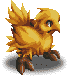
\includegraphics[width=0.17\textwidth]{./art/monsters/chocobo.png}}
{
		HP: & \hfill 23 & MP: & \hfill 24\\
STR: & \hfill 2 & DEF: & \hfill 1 \\
MAG: & \hfill 3 & RES: & \hfill 2 \\
AGI: & \hfill 4 & Size: & \hfill M\\
}
{
	\textbf{Beak}: 1d DMG \hfill \textbf{Drops:} 250 Gil
	
	\mspell{Cure}{4}{1r}{Single}{3u}{
		The target regains 2d HP.
	}{}		
	\mspell{Esuna}{8}{1r}{Single}{3u}{
	You remove all status effects from the target except \hyperlink{status}{KO}.
}{}		
	%\vspace{0.1cm} \hrule \vspace{0.1cm} 
	%\emph{"Kweh." -- Chocobo}
}
 
\monster{Bomb}{3}{
\includegraphics[width=0.17\textwidth]{./art/monsters/bomb.png}}
{
	HP: & \hfill 22 & MP: & \hfill 12\\
	STR: & \hfill 3 & DEF: & \hfill 2 \\
	MAG: & \hfill 2 & RES: & \hfill 1 \\
	AGI: & \hfill 3 & Size: & \hfill M\\
}
{
	\textbf{Tackle}: 1d DMG \hfill \textbf{Drops:} 200 Gil \\
	\textbf{Resilient}:\fire \hfill \textbf{Weak}:\ice 

	\mtech{Self-Destruct}{0}{1r}{2u}{Self}{
		Inflict \hyperlink{status}{KO} on yourself to deal 6d \hyperlink{type}{fire} damage to everyone within the target area.
	}{\fire}		
	%\vspace{0.1cm} \hrule \vspace{0.1cm} 
	%\emph{"Run run, or you'll be well done!" -- Kefka}
} 
\monster{Blue Flan}{3}{
\includegraphics[width=0.25\textwidth]{./art/monsters/flan.png}}
{
	HP: & \hfill 12 & MP: & \hfill 30\\
	STR: & \hfill 0 & DEF: & \hfill 6 \\
	MAG: & \hfill 5 & RES: & \hfill 1 \\
	AGI: & \hfill 1 & Size: & \hfill M\\
}
{
	\textbf{Tackle}: 1d DMG \hfill 	\textbf{Drops:} 200 Gil \\
	\textbf{Resilient}:\ice \hspace*{\fill} \textbf{Weak}:\fire 
	
	\mspell{Blizzard}{4}{1r}{Single}{3u}{
		You deal 2d \hyperlink{type}{ice} damage to the target.
	}{\ice}		
	%\vspace{0.1cm} \hrule \vspace{0.1cm} 
	%\emph{"Icing on the cake!" -- Lulu}
}
 
\monster{Abeja Asesina}{3}{
\includegraphics[width=0.15\textwidth]{./art/monsters/killerbee.png}}
{
 PV: & \hfill 18 & PM: & \hfill 0 \\
 FUE: & \hfill 2 & DEF: & \hfill 1 \\
 MAG: & \hfill 1 & RES: & \hfill 3 \\
 AGI: & \hfill 3 & Tamaño: & \hfill P\\
}
{
 \textbf{Aguijón}: 2d de daño \hfill \textbf{Botín:} 150 Gil \\
 \textbf{Inmune}:\poison \mpassive{Toque Venenoso}{
 Siempre que hagas un \hyperlink{action}{Ataque} con éxito, el objetivo debe hacer una tirada con DC 8. Si falla, queda \hyperlink{status}{Envenenado} por 3 turnos.
	}
	%\vspace{0.1cm} \hrule \vspace{0.1cm} 
 %\emph{"¡No me gusta tener criaturas de bajo vuelo tratando de matarme!"\\ -- Sazh}
}  

%%%%%%%%%%%%%%L4%%%%%%%%%%%%%%
\monster{Gárgola}{4}{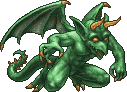
\includegraphics[width=0.23\textwidth]{./art/monsters/gargoyle.png}}
{
 PV: & \hfill 35 & PM: & \hfill 0\\
 FUE: & \hfill 4 & DEF: & \hfill 6 \\
 MAG: & \hfill 0 & RES: & \hfill 1 \\
 AGI: & \hfill 2 & Tamaño: & \hfill M\\
}
{
 \textbf{Garra}: 2d de daño \hfill \textbf{Botín:} 300 Gil \\
 \textbf{Resistencia}:\earth \hfill \textbf{Debilidad}:\water %\vspace{0.1cm} \hrule \vspace{0.1cm} 
 %\emph{"Ese muchacho no es muy optimista." -- Alisaie}
}
\monster{Ahriman}{4}{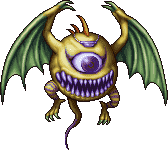
\includegraphics[width=0.21\textwidth]{./art/monsters/ahriman.png}}
{
	HP: & \hfill 28 & MP: & \hfill 24\\
	STR: & \hfill 0 & DEF: & \hfill 1 \\
	MAG: & \hfill 4 & RES: & \hfill 4 \\
	AGI: & \hfill 4 & Size: & \hfill S\\
}
{
	\textbf{Beam}: 2d DMG, 3u Range \hfill \textbf{Drops:} 350 Gil 
	
	\mtech{Eerie Soundwave}{6}{1r}{Single}{3u}{
		The target makes a DC 8 check and suffers  2d damage and \hyperlink{status}{Silence} for 3 rounds upon failure.
	}{\silence}		
	%\vspace{0.1cm} \hrule \vspace{0.1cm} 
	%\emph{"There are none who can stop me in all of creation! You, too shall fall before me!" -- Ahriman}	
} 
\monster{Antoleón}{4}{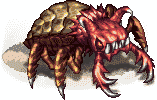
\includegraphics[width=0.26\textwidth]{./art/monsters/antlion.png}}
{
 PV: & \hfill 40 & PM: & \hfill 16\\
 FUE: & \hfill 3 & DEF: & \hfill 3 \\
 MAG: & \hfill 0 & RES: & \hfill 1 \\
 AGI: & \hfill 3 & Tamaño: & \hfill M\\
}
{
 \textbf{Mordida}: 2d de daño \hfill \textbf{Botín:} 300 Gil \\
 \textbf{Resistencia}:\earth \hfill \textbf{Inmune}:\blind 
 
 \mtech{Tormenta de Arena}{8}{1t}{3u}{Tú}{
 Todos los enemigos que se encuentren en el área de efecto deben hacer una tirada con DC 9. Si fallan, reciben 3d de daño de \hyperlink{type}{Tierra} y quedan \hyperlink{status}{Ciegos} por 3 turnos. }{\earth \blind} %\vspace{0.1cm} \hrule \vspace{0.1cm} 
 %\emph{"No ha problema. Los anteleones son bastante dóciles." -- Edward}
}
 
\monster{Diablillo}{4}{
\includegraphics[width=0.13\textwidth]{./art/monsters/imp.png}}
{
 PV: & \hfill 30 & PM: & \hfill 50 \\
 FUE: & \hfill 1 & DEF: & \hfill 2 \\
 MAG: & \hfill 5 & RES: & \hfill 4 \\
 AGI: & \hfill 4 & Tamaño: & \hfill P\\
}
{
 \textbf{Garra}: 2d de daño \hfill \textbf{Botín:} 400 Gil \\
 \textbf{Resistencia}:\dark \mspell{Confusión}{10}{1t}{Único}{5u}{
 El objetivo hace una tirada con DC 8. Si falla, queda bajo tu control en su próximo turno. Puedes ordenarle que se mueva y que \hyperlink{action}{Ataque} a cualquier objetivo que elijas, incluyendo a él mismo. }{} %\vspace{0.1cm} \hrule \vspace{0.1cm} 
 %\emph{"Quizás Dios perdonaría a un horrible pedazo de basura como tú... ¡pero yo no!" -- Cid}
} 
\monster{Mummy}{4}{
\includegraphics[width=0.14\textwidth]{./art/monsters/mummy.png}}
{
	HP: & \hfill 38 & MP: & \hfill 0\\
	STR: & \hfill 2 & DEF: & \hfill 3 \\
	MAG: & \hfill 0 & RES: & \hfill 1 \\
	AGI: & \hfill 2 & Size: & \hfill M\\
}
{
	\textbf{Bite}: 2d DMG \hfill \textbf{Drops:} 350 Gil  \\
	\textbf{Immune}:\poison\sleep \hfill \textbf{Weak}:\fire 
	
	\mpassive{Zombietouch}{Whenever you successfully \hyperlink{action}{Attack} a target he makes a DC 8 check and suffers \hyperlink{status}{Zombie} for 1~hour upon failure.}
	\mpassive{Undead}{You permamently suffer the \hyperlink{status}{Zombie} status.}
	%\vspace{0.1cm} \hrule \vspace{0.1cm} 
	%\emph{"I don't like two-legged things." -- Red XIII}
}		 

%%%%%%%%%%%%%%L5%%%%%%%%%%%%%%
\monster{Drago}{5}{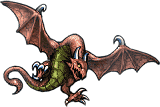
\includegraphics[width=0.25\textwidth]{./art/monsters/wyvern.png}}
{
 PV: & \hfill 45 & PM: & \hfill 50 \\
 FUE: & \hfill 3 & DEF: & \hfill 3 \\
 MAG: & \hfill 2 & RES: & \hfill 3 \\
 AGI: & \hfill 3 & Tamaño: & \hfill M\\
}
{
 \textbf{Garra}: 2d de daño \hfill \textbf{Botín:} 400 Gil 
 
 \mspell{Aero}{8}{1t}{Único}{4u}{
 Infliges 3d de daño de \hyperlink{type}{Viento} al objetivo. }{\wind}
 \mpassive{Zambullida}{
 Siempre que realices un \hyperlink{action}{Ataque} sobre un objetivo, él debe hacer una tirada con DC 6. Si falla, queda \hyperlink{status}{Inmóvil} por 1 turno.
	}
	%\vspace{0.1cm} \hrule \vspace{0.1cm} 
 %\emph{"Y así, Laguna corre por su preciada vida." -- Kiros}
} 
\monster{Quimera}{5}{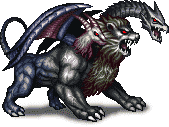
\includegraphics[width=0.26\textwidth]{./art/monsters/chimera.png}}
{
 PV: & \hfill 60 & PM: & \hfill 90\\
 FUE: & \hfill 1 & DEF: & \hfill 2 \\
 MAG: & \hfill 4 & RES: & \hfill 3 \\
 AGI: & \hfill 3 & Tamaño: & \hfill M\\
}
{
 \textbf{Garra}: 2d de daño \hfill \textbf{Botín:} 500 Gil\\
 \textbf{Resistencia}:\fire \ice \lightning 
 
 \mspell{Piro++}{12}{2t}{Único}{5u}{Inflijes 6d de daño de \hyperlink{type}{Fuego} al objetivo. }{\fire} 
 \mspell{Hielo++}{12}{2t}{Único}{5u}{Inflijes 6d de daño de \hyperlink{type}{Hielo} al objetivo. }{\ice} 
 \mspell{Electro++}{12}{2t}{Único}{5u}{Inflijes 6d de daño de \hyperlink{type}{Eléctrico} al objetivo.}{\lightning}
 %\vspace{0.1cm} \hrule \vspace{0.1cm} 
 %\emph{"Genial, ahora estoy luchando contra cuentos de hadas." -- Lightning}
} 
\monster{Gigante}{5}{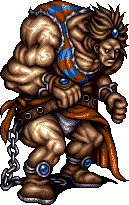
\includegraphics[width=0.13\textwidth]{./art/monsters/gigas.png}}
{
 PV: & \hfill 70 & PM: & \hfill 50\\
 FUE: & \hfill 6 & DEF: & \hfill 4 \\
 MAG: & \hfill 1 & RES: & \hfill 2 \\
 AGI: & \hfill 1 & Tamaño: & \hfill G\\
}
{
 \textbf{Puño}: 2d de daño, 2u Alcance \hfill \textbf{Botín:} 450 Gil
 
 \mtech{Cabezazo}{10}{1t}{Único}{2u}{Infliges 6d de daño al objetivo y lo empujas 3u hacia atrás.}{}
 %\vspace{0.1cm} \hrule \vspace{0.1cm} 
 %\emph{"¡Puaj! ¡Odio a los hombres musculosos! ¿Son los refuerzos o qué?" -- Ultros}
} 
\friendly{Magic Pot}{5}{
\includegraphics[width=0.12\textwidth]{./art/monsters/magicpot.png}}
{
	HP: & \hfill 1 & MP: & \hfill 1\\
	STR: & \hfill 0 & DEF: & \hfill 99 \\
	MAG: & \hfill 0 & RES: & \hfill 99 \\
	AGI: & \hfill 1 & Size: & \hfill S\\
}
{
	\textbf{Immune}: \hyperlink{status}{All Status Effects} \hfill 	\textbf{Drops:} 1000 Gil 
	
	\mreaction{Gimme!}{
		When given a beneficial \hyperlink{item}{item} you disappear (\hyperlink{status}{KO}), dropping Gil.
		Otherwise, you make a DC 8 check and upon failure you suffer \hyperlink{status}{KO} to deal 8d damage in 3u around you, dropping no Gil.
	}
	%%%%%%%%%%%%%%%%%%%%%%%%%%%%%%%%%%%%%%%%%%
	%\vspace{0.1cm} \hrule \vspace{0.1cm} 
	%\emph{"Gimme Elixir!" -- Magic Pot}
}
\monster{Cactuar}{5}{
\includegraphics[width=0.14\textwidth]{./art/monsters/cactuar.png}}
{
	HP: & \hfill 20 & MP: & \hfill 40\\
	STR: & \hfill 1 & DEF: & \hfill 1 \\
	MAG: & \hfill 4 & RES: & \hfill 10 \\
	AGI: & \hfill 6 & Size: & \hfill S\\
}
{
	\textbf{Tackle:} 1d DMG \hfill \textbf{Drops:} 1000 Gil  \\
	\textbf{Immune}:\sleep \blind 
	
	\mtech{1000 Needles}{10}{0r}{Single}{1u}{
		You deal 10d damage to the target.
	}{}	
	\mpassive{Flee}{When running away from enemies you can move 2u further than usual.}	
	%%%%%%%%%%%%%%%%%%%%%%%%%%%%%%%%%%%%%%%%%%
	\vspace{0.1cm} \hrule \vspace{0.1cm} 
	"Needles, I hate needles!" -- Rikku
}
 

%%%%%%%%%%%%%%L6%%%%%%%%%%%%%%
\monster{Mindflayer}{6}{
\includegraphics[width=0.20\textwidth]{./art/monsters/mindflayer.png}}
{
	HP: & \hfill 65 & MP: & \hfill 130 \\
	STR: & \hfill 1 & DEF: & \hfill 2 \\
	MAG: & \hfill 6 & RES: & \hfill 7 \\
	AGI: & \hfill 2 & Size: & \hfill M\\
}
{
	\textbf{Staff}: 1d DMG \hfill \textbf{Drops:} 700 Gil \\
	\textbf{Weak}:\lightning \hfill	\textbf{Resilient}:\water \\
	\textbf{Immune}:\poison\silence\sleep
	
	\mspell{Waterga}{14}{2r}{Single}{5u}{
		You deal 8d \hyperlink{type}{water} damage to the target.  
	}{\water}
	\mtech{Mind Blast}{20}{1r}{2u}{5u}{
		All enemies in the target area suffer 4d \hyperlink{type}{dark} damage and \hyperlink{status}{Immobile} for 1 round.
	}{\immobile \dark}	
	%\vspace{0.1cm} \hrule \vspace{0.1cm} 
	%\emph{"Why do I get the feeling this is not the safest place to be...?" -- Luneth}	
}
 
\monster{Medusa}{6}{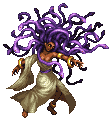
\includegraphics[width=0.18\textwidth]{./art/monsters/medusa.png}}
{
	HP: & \hfill 70 & MP: & \hfill 110\\
	STR: & \hfill 3 & DEF: & \hfill 4 \\
	MAG: & \hfill 5 & RES: & \hfill 4 \\
	AGI: & \hfill 3 & Size: & \hfill M\\
}
{
	\textbf{Hair}: 2d DMG \hfill \textbf{Drops:} 750 Gil \\
	\textbf{Resilient}:\earth\lightning \hfill \textbf{Weak}:\water \\
	\textbf{Immune}:\poison\sleep\immobile 
	
	
	\mtech{Gaze}{15}{1r}{3u (front)}{Self}{Everyone in the target area makes a DC~8 check~and suffers \hyperlink{status}{Immobile} for 3 rounds upon failure.}{\immobile}	
	\mspell{Thundaga}{12}{2r}{Single}{5u}{You deal 6d \hyperlink{type}{lightning} damage to the target.}{\lightning}
	\vspace{0.1cm} \hrule \vspace{0.1cm} 
	"Just lookin' at you is makin' me sober." -- Reno
} 
\monster{Lamia}{6}{
\includegraphics[width=0.24\textwidth]{./art/monsters/lamia.png}}
{
 PV: & \hfill 70 & PM: & \hfill 100 \\
 FUE: & \hfill 2 & DEF: & \hfill 3 \\
 MAG: & \hfill 6 & RES: & \hfill 5 \\
 AGI: & \hfill 3 & Tamaño: & \hfill M\\
}
{
 \textbf{Bofetada}: 2d de daño \hfill \textbf{Botín:} 800 Gil \\
 \textbf{Resistencia}:\water \hfill \textbf{Débil}:\lightning \\
 \textbf{Inmune}:\poison\sleep\silence \mspell{Rana}{16}{2t}{Único}{5u}{
 El objetivo debe hacer una tirada con DC 8. Si falla, queda convertido en una rana por 5 turnos o hasta que reciba daño. Mientras esté convertido en rana, el objetivo no puede hablar ni realizar ninguna acción y solo puede moverse 1u por turno. }{} \mreaction{Encantar}{
 Siempre que un enemigo te golpee con éxito con un \hyperlink{action}{Ataque}, debe hacer una tirada con DC~6.  Si falla, puedes ordenarle que realice las acciones y movimientos que elijas y debe seguir esas órdenes en su próximo turno. 
	}
	%\vspace{0.1cm} \hrule \vspace{0.1cm} 
 %\emph{"¿¡Ranas!? ¡Odio las ranas! ¡No me conviertas en una!" -- Refia}
} 
\monster{Gigante de Hierro}{6}{
\includegraphics[width=0.16\textwidth]{./art/monsters/irongiant.png}}
{
 PV: & \hfill 80 & PM: & \hfill 48 \\
 FUE: & \hfill 5 & DEF: & \hfill 5 \\
 MAG: & \hfill 0 & RES: & \hfill 4 \\
 AGI: & \hfill 3 & Tamaño: & \hfill G\\
}
{
 \textbf{Espada}: 3d de daño, 2u Alcance \hfill \textbf{Botín:} 500 Gil %\\
 \textbf{Resilient}:\physical
 \mtech{Arrasar}{12}{1t}{3u (frente)}{Tú}{Realiza un \hyperlink{action}{Ataque} contra todos los enemigos dentro del área de efecto.}{}
} 

%%%%%%%%%%%%%%L7%%%%%%%%%%%%%%
\monster{\hypertarget{malboro}{Malboro}}{7}{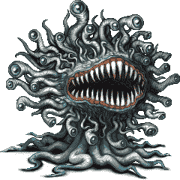
\includegraphics[width=0.21\textwidth]{./art/monsters/malboro.png}}
{
 PV: & \hfill 100 & PM: & \hfill 100 \\
 FUE: & \hfill 2 & DEF: & \hfill 4 \\
 MAG: & \hfill 5 & RES: & \hfill 7 \\
 AGI: & \hfill 2 & Tamaño: & \hfill G\\
}
{
 \textbf{Tentáculo}: 2d de daño \hfill \textbf{Botín:} 1000 Gil \\
 \textbf{Inmune}: \hyperlink{status}{Todos los Estados Alterados} \hfill \textbf{Debilidad}:\fire 
 
 \mtech{Mal Aliento}{20}{1t}{3u (frente)}{Tú}{
 Todos los enemigos en el área de efecto hacen una tirada con DC 8. Si fallan, quedan \hyperlink{status}{Dormidos},   \hyperlink{status}{Envenenados}, en \hyperlink{status}{Silencio} y \hyperlink{status}{Ciegos} por 3 turnos. }{\sleep \poison \silence \blind} \mtech{Jugo Gástrico}{10}{1t}{2u}{8u}{
 Todos los enemigos dentro del área de efecto reciben 5d de daño y deben hacer una tirada con DC 8. Todos los que fallen reciben  \hyperlink{status}{disFUE} y \hyperlink{status}{disMAG} por 5 turnos. }{\destr \demag} %\vspace{0.1cm} \hrule \vspace{0.1cm} 
 %\emph{"Eso parece una boca. ¿¡Es esa su cara!?" -- Prompto}
}
 
\monster{Zu}{7}{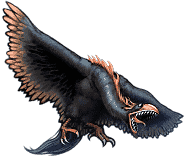
\includegraphics[width=0.23\textwidth]{./art/monsters/zu.png}}
{
 PV: & \hfill 160 & PM: & \hfill 100 \\
 FUE: & \hfill 7 & DEF: & \hfill 5 \\
 MAG: & \hfill 3 & RES: & \hfill 6 \\
 AGI: & \hfill 2 & Tamaño: & \hfill G\\
}
{
 \textbf{Garra}: 3d de daño \hfill \textbf{Botín:} 1000 Gil \\
 \textbf{Inmune}:\poison \sleep \silence \mtech{Tornado}{20}{1t}{9u (línea)}{Tú}{
 Creas un tornado de 2u de diámetro que se mueve 3u en línea por turno. El tornado dura 3 turnos. Cualquiera que entre en contacto con el tornado (excepto tú) sufre 4d de daño de \hyperlink{type}{Viento} y queda \hyperlink{status}{Inmóvil} por 1 turno. }{\wind \immobile} %\mpassive{Auto-Regen}{
 % Recuperas 25 PV al principio de cada turno. %} %\vspace{0.1cm} \hrule \vspace{0.1cm} 
 %\emph{"¿Cómo puede un ave ser tan grande?" -- Tidus} 
}
 
\monster{Cerberus}{7}{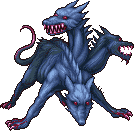
\includegraphics[width=0.21\textwidth]{./art/monsters/cerberus.png}}
{
	HP: & \hfill 120 & MP: & \hfill 110 \\
	STR: & \hfill 5 & DEF: & \hfill 3 \\
	MAG: & \hfill 6 & RES: & \hfill 4 \\
	AGI: & \hfill 3 & Size: & \hfill L\\
}
{
	\textbf{Bite}: 3d DMG  \\
	\textbf{Resilient}:\fire\ice\lightning \hfill \textbf{Drops:} 1000 Gil 
	%\hfill \textbf{Weak}:\lightning 
	%\textbf{Immune}:\poison\sleep
	
	\mspell{Firaga}{12}{2r}{Single}{5u}{You deal 6d \hyperlink{type}{fire} damage to the target. }{\fire}
	\mpassive{Triple Triad}{You can perform each action on up to 3 different targets within its range simultaneously.}
	%\vspace{0.1cm} \hrule \vspace{0.1cm} 
	%\emph{"So, you've managed to reach these depths. I commend you. But your journey ends here, I'm afraid." -- Cerberus}
} 
\monster{\hypertarget{abyssworm}{Sand Worm}}{7}{
\includegraphics[width=0.21\textwidth]{./art/monsters/abyssworm.png}}
{
	HP: & \hfill 150 & MP: & \hfill 120 \\
	STR: & \hfill 7 & DEF: & \hfill 4 \\
	MAG: & \hfill 5 & RES: & \hfill 6 \\
	AGI: & \hfill 1 & Size: & \hfill L\\
}
{
	\textbf{Acid}: 3d DMG, 3u Range \hfill \textbf{Drops:} 1000 Gil \\
	\textbf{Immune}:\poison \sleep 
	
	\mspell{Quake}{22}{2r}{4u}{8u}{
		You deal 8d \hyperlink{type}{earth} damage to everyone in the target area. 
	}{\earth}	
	\mtech{Inhale}{20}{1r}{Single}{3u}{
		You inhale the target, removing him from the battle. 
		At the beginning of every turn he may try to free himself by passing a DC 9 check.
	}{}		
	%\vspace{0.1cm} \hrule \vspace{0.1cm} 
	%\emph{"Ah, where’s the early bird when you need one?" -- Wakka}	
}
 
\monster{Zombie Dragon}{7}{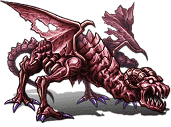
\includegraphics[width=0.28\textwidth]{./art/monsters/zombiedragon.png}}
{
	HP: & \hfill 125 & MP: & \hfill 80\\
	STR: & \hfill 6 & DEF: & \hfill 5 \\
	MAG: & \hfill 0 & RES: & \hfill 3 \\
	AGI: & \hfill 2 & Size: & \hfill L\\
}
{
	\textbf{Bite}: 3d DMG, 2u Range \hfill	\textbf{Drops:} 900 Gil  \\
	\textbf{Immune}:\ko\poison\sleep\silence \hfill  \textbf{Weak}:\holy
  
	
	\mtech{Poison Breath}{10}{1r}{3u (front)}{Self}{Everyone in the target area suffers 4d damage, makes a DC~8 check~and suffers \hyperlink{status}{Poison} for 3 rounds upon failure.}{\poison}	
	\mreaction{Regenerate}{
		When reduced below 50 HP, you become unable to move or act.
		You regenerate 50 HP on each turn for 3 rounds after which you can act and move again.  
		This effect can only be used once per battle.
	}	
	\mpassive{Undead}{You permamently suffer the \hyperlink{status}{Zombie} status.}
	%\vspace{0.1cm} \hrule \vspace{0.1cm} 
	%\emph{"Don't eat me! I won't taste good!" -- Eiko}
}
 

%%%%%%%%%%%%%%L8%%%%%%%%%%%%%%
\monster{Behemoth}{8}{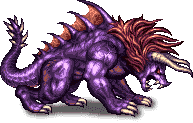
\includegraphics[width=0.32\textwidth]{./art/monsters/behemoth.png}}
{
 PV: & \hfill 200 & PM: & \hfill 250 \\
 FUE: & \hfill 8 & DEF: & \hfill 5 \\
 MAG: & \hfill 5 & RES: & \hfill 4 \\
 AGI: & \hfill 3 & Tamaño: & \hfill G\\
}
{
 \textbf{Garra}: 3d de daño, 2u Alcance \hfill \textbf{Botín:} 1500 Gil \\
 \textbf{Inmune}:\poison \silence 
 
 \mspell{Llamarada}{30}{3t}{Único}{5u}{Infliges 9d+15 de daño de \hyperlink{type}{Fuego} al objetivo. }{\fire}
 \mtech{Embestida}{20}{0t}{Único}{2u}{Infliges 10d de daño al objetivo y lo haces volar 3u por el aire durante 1 turno. }{} 
 \mreaction{Contraataque}{Siempre que seas el objetivo de la acción de un enemigo que se encuentre a 2u de ti, inmediatamente haz un \hyperlink{action}{Ataque} sobre él.}
%\vspace{0.1cm} \hrule \vspace{0.1cm} 
%\emph{"¿Suficientemente grande para ti?" -- Gladio} 
}
 
\monster{Ochu}{8}{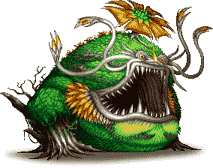
\includegraphics[width=0.27\textwidth]{./art/monsters/ochu.png}}
{
	HP: & \hfill 180 & MP: & \hfill 100 \\
	STR: & \hfill 7 & DEF: & \hfill 5 \\
	MAG: & \hfill 6 & RES: & \hfill 4 \\
	AGI: & \hfill 1 & Size: & \hfill L\\
}
{
	\textbf{Vines}: 3d DMG, 3u Range \hfill \textbf{Drops:} 1500 Gil \\
	\hfill \textbf{Immune}:\poison \sleep \blind 
	
	\mtech{Pollen}{15}{1r}{5u}{Self}{
		All enemies in the target area make a DC 8 check and suffer \hyperlink{status}{Sleep} \& \hyperlink{status}{Poison} for 3 rounds on failure.
	}{\sleep \poison}	
	%\vspace{0.1cm} \hrule \vspace{0.1cm} 
	%\emph{"The Ochu is no garden variety fiend. We could throw a hundred Crusaders at it and still lose." -- Luzzu}
} 
\monster{Muro Demoníaco}{8}{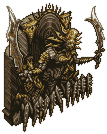
\includegraphics[width=0.17\textwidth]{./art/monsters/demonwall.png}}
{
 PV: & \hfill 250 & PM: & \hfill 200 \\
 FUE: & \hfill 9 & DEF: & \hfill 6 \\
 MAG: & \hfill 5 & RES: & \hfill 6 \\
 AGI: & \hfill 2 & Tamaño: & \hfill G\\
}
{
 \textbf{Espadas}: 3d de daño, 2u Alcance \hfill \textbf{Botín:} 2000 Gil \\
 \textbf{Inmune}: \hyperlink{status}{Todos los estados alterados} 
 
 \mtech{Morfeo++}{24}{2t}{2u}{5u}{
 Todos los enemigos que se encuentren en el área de efecto hacen una tirada con DC 8. Si fallan, \linebreak quedan \hyperlink{status}{Dormidos}. 
	}{\sleep} \mtech{Arremetida de Muro}{20}{1t}{10u (línea)}{Tú}{
 Arremetes hasta 10u hacia adelante en línea recta, infligiendo 8d de daño a todos los que estén en tu camino y los haces retroceder 3u. Si un enemigo queda aplastado entre ti y un muro, instantáneamente \linebreak pasan a estar \hyperlink{status}{KO}. 
}{\ko} 
\mpassive{Giro Brusco}{
 Cada vez que cambias de dirección, todos los que se encuentren a 2u reciben 6d de daño, pero no puedes realizar una acción en el mismo turno.
	}
	\vspace{0.1cm} \hrule \vspace{0.1cm} 
 "Como si las puertas asesinas no fueran suficientes..." -- Rydia
}

 
\monster{Dragón Rojo}{8}{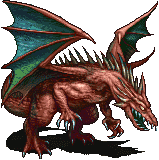
\includegraphics[width=0.2\textwidth]{./art/monsters/reddragon.png}}
{
 PV: & \hfill 225 & PM: & \hfill 250 \\
 FUE: & \hfill 6 & DEF: & \hfill 4 \\
 MAG: & \hfill 5 & RES: & \hfill 4 \\
 AGI: & \hfill 3 & Tamaño: & \hfill G\\
}
{
 \textbf{Mordida}: 3d de daño \hfill \textbf{Botín:} 1500 Gil \\
 \textbf{Resistencia}:\fire \hfill \textbf{Débil}:\ice \\
 \textbf{Inmune}:\sleep\blind\immobile \mspell{Fulgor}{30}{3t}{Único}{5u}{Infliges 9d+15 de daño de \hyperlink{type}{Fuego} al objetivo. }{\fire}
 \mtech{Llamarada}{22}{1t}{3u (frente)}{Tú}{
 Infliges 8d de daño de \hyperlink{type}{Fuego} a todos los enemigos que se encuentren dentro del área de efecto. }{\fire}
 \mpassive{Coletazo}{ Cuando realices un \hyperlink{action}{Ataque}, puedes elegir atacar a todos los enemigos que se encuentren a 1u de ti.}
	%\vspace{0.1cm} \hrule \vspace{0.1cm} 
 %\emph{"¡No sabía que un dragón tan poderoso existía en este universo!" -- Kain} 
} 

%%%%%%%%%%%%%%L9%%%%%%%%%%%%%%
\monster{Tomberi}{9}{
\includegraphics[width=0.26\textwidth]{./art/monsters/tonberry.png}}
{
 PV: & \hfill 280 & PM: & \hfill 100\\
 FUE: & \hfill 12 & DEF: & \hfill 6 \\
 MAG: & \hfill 3 & RES: & \hfill 5 \\
 AGI: & \hfill 2 & Tamaño: & \hfill P\\
}
{
 \textbf{Cuchillo}: 4d de daño \hfill \textbf{Botín:} 4000 Gil \\
 \textbf{Inmune}:\poison \blind \sleep \mpassive{Rencor}{
 Cada vez que \hyperlink{status}{Ataques} a un enemigo, este debe hacer una tirada con DC 7. Si falla, queda \hyperlink{status}{KO}. } \mreaction{Karma}{Siempre que un enemigo que se encuentre a más de 3u de ti reduzca tus PV, hazle 8d de daño \hyperlink{type}{Oscuro}. }
	\vspace{0.1cm} \hrule \vspace{0.1cm} 
 "Un cuchillo de cocina. Me pregunto si lo que quiere es una batalla culinaria." -- Ignis } 
\monster{Kraken}{9}{
\includegraphics[width=0.23\textwidth]{./art/monsters/kraken.png}}
{
	HP: & \hfill 320 & MP: & \hfill 400 \\
	STR: & \hfill 7 & DEF: & \hfill 5 \\
	MAG: & \hfill 11 & RES: & \hfill 7 \\
	AGI: & \hfill 2 & Size: & \hfill L\\
}
{
	\textbf{Tentacle}: 4d DMG, 2u range \hfill \textbf{Drops:} 2000 Gil \\
	\textbf{Resilient}:\water\ice \hfill \textbf{Immune}:\poison\sleep\blind 
	
	\mspell{Waterga}{14}{2r}{Single}{5u}{You deal 8d \hyperlink{type}{water} damage to the target. }{\water}	
	\mtech{Ink}{22}{1r}{2u}{5u}{
		All enemies within the target area make a DC 8 check and suffer \hyperlink{status}{Blind} and 4d damage upon failure. 
	}{\blind}
	\mpassive{Multiattack}{Whenever you choose to \hyperlink{action}{Attack}, you can target all enemies within range at once.}
	%\vspace{0.1cm} \hrule \vspace{0.1cm} 
	%\emph{"I am the Kraken... Your presence is forbidden!"}
} 
\monster{Adamantoise}{9}{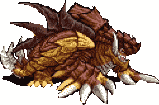
\includegraphics[width=0.31\textwidth]{./art/monsters/adamantoise.png}}
{
	HP: & \hfill 350 & MP: & \hfill 400 \\
	STR: & \hfill 10 & DEF: & \hfill 7 \\
	MAG: & \hfill 8 & RES: & \hfill 6 \\
	AGI: & \hfill 1 & Size: & \hfill L\\
}
{
	\textbf{Trample}: 4d DMG, 2u Target \hfill \textbf{Drops:} 3000 Gil \\
	\textbf{Immune}:\poison \silence \hfill \textbf{Resilient}:\earth
	
	\mspell{Ultima}{45}{3r}{3u}{5u}{
		You deal 10d+20 \hyperlink{type}{dark} damage to all enemies in the target area.  
	}{\dark}	
	\mtech{Roar}{20}{1r}{2u}{5u}{
		All enemies within the target area make a DC 9 check and suffer \hyperlink{status}{Immobile} for 3 rounds upon failure. 
	}{\immobile}	
	\mreaction{Vigor}{
		Whenever you suffer damage while concentrating, the cast time of the ability you are preparing is reduced by 1 round.  
	}	
	%\vspace{0.1cm} \hrule \vspace{0.1cm} 
	%\emph{"Not our lucky day." -- Fang}	
}
 
\monster{Lich}{9}{
\includegraphics[width=0.20\textwidth]{./art/monsters/lich.png}}
{
	HP: & \hfill 300 & MP: & \hfill 500\\
	STR: & \hfill 4 & DEF: & \hfill 5 \\
	MAG: & \hfill 12 & RES: & \hfill 8 \\
	AGI: & \hfill 2 & Size: & \hfill L\\
}
{
	\textbf{Beam}: 4d DMG, 5u Range \hfill \textbf{Drops:} 5000 Gil  \\
	\textbf{Immune}: \hyperlink{status}{All Status Effects}\\
	\textbf{Weak}:\holy \hfill \textbf{Resilient}:\dark 
	
	\mspell{Zombify}{22}{1r}{2u}{5u}{
		Everyone in the target makes a DC 8 check and suffers \hyperlink{status}{Zombie} for 1 hour upon failure.
	}{\zombie}	
	\mspell{Poisonga}{24}{1r}{2u}{5u}{
		Everyone in the target area makes a DC 8 check and suffers \hyperlink{status}{Poison} for 3 rounds upon failure.
	}{\poison}	
	\mspell{Doom}{36}{1r}{Single}{5u}{
		The target makes a DC 8 check and suffers \hyperlink{status}{KO} after 3 rounds upon failure.
	}{\ko}	
	\mpassive{Greater Undead}{
		You permamently suffer \hyperlink{status}{Zombie}, but are immune to effects that cause or cure \hyperlink{status}{KO}.
	}
	%\vspace{0.1cm} \hrule \vspace{0.1cm} 
	%\emph{"Was that Death himself? I felt a sudden dread course through my veins..." -- Ceodore}
}

 

%%%%%%%%%%%%%%L10%%%%%%%%%%%%%%
\monster{Caos}{10}{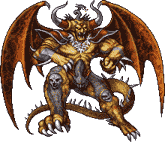
\includegraphics[width=0.23\textwidth]{./art/monsters/chaos.png}}
{
 PV: & \hfill 400 & PM: & \hfill 700 \\
 FUE: & \hfill 8 & DEF: & \hfill 8 \\
 MAG: & \hfill 10 & RES: & \hfill 7 \\
 AGI: & \hfill 4 & Tamaño: & \hfill G\\
}
{
 \textbf{Haz}: 5d de daño, 3u Alcance \hfill \textbf{Botín:} 10000 Gil \\
 \textbf{Inmune}: \hyperlink{status}{Todos los Estados Alterados} \\
 \textbf{Resistencia}:\dark\fire \mspell{Artema}{45}{3t}{3u}{5u}{
 Infliges 10d+10 de daño \hyperlink{type}{Oscuro} solo a los enemigos que se encuentren en el área de efecto. }{\dark} \mspell{Cura+++}{30}{2t}{3u}{5u}{
 Todos los aliados que se encuentren en el área de efecto recuperan 8d+10 de sus PV. }{} \mspell{Piro+++}{28}{2t}{3u}{8u}{
 Infliges 8d+10 de daño de \hyperlink{type}{Fuego} a todos los que se encuentren en el área de efecto. }{\fire}
 \mpassive{Toque Caótico}{
 Siempre que hagas un \hyperlink{action}{Ataque} con éxito, el objetivo debe hacer una tirada con DC 8. Si falla, sufre \hyperlink{status}{Veneno}, \hyperlink{status}{Ciego} y \hyperlink{status}{Silencio} por 3 turnos.
	}
 \mreaction{Acelerar}{
 Siempre que recibas daño, puedes hacer una tirada con DC 6. Si tienes éxito, tienes un turno adicional inmediatamente después del atacante. Este efecto no cambia el orden habitual de los turnos y solo puede utilizarse una vez por turno.
	}
	\vspace{0.1cm} \hrule \vspace{0.1cm} 
 "Pero renaceré una vez más. Así que aunque muera una y otra vez, yo regresaré. ¡Renacido en este ciclo infinito que he creado!" -- Caos }
 
\monster{Shinriu}{10}{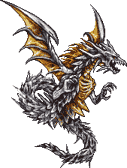
\includegraphics[width=0.16\textwidth]{./art/monsters/shinryu.png}}
{
 PV: & \hfill 500 & PM: & \hfill 800 \\
 FUE: & \hfill 12  & DEF: & \hfill 8 \\
 MAG: & \hfill 14 & RES: & \hfill 9 \\
 AGI: & \hfill 4 & Tamaño: & \hfill G\\
}
{
 \textbf{Cola}: 5d de daño, 4u Alcance \hfill \textbf{Botín:} 25000 Gil\\
 \textbf{Inmune}: \hyperlink{status}{Todos los Estados Alterados} \mspell{Ola Sísmica}{35}{2t}{12u (frente)}{Tú}{
 Todos los enemigos en el área de efecto reciben 9d+10 de daño de \hyperlink{type}{Agua} y quedan \hyperlink{status}{Inmóviles} por 2 turnos. }{\water \immobile} \mspell{Rayo Atómico}{45}{2t}{8u}{Tú}{
 Todos los enemigos en el área de efecto reciben 8d+9 de daño de \hyperlink{type}{Fuego} y quedan \hyperlink{status}{Envenenados} por 3 turnos. }{\fire \poison} \mpassive{Adaptar Elemento}{
 Al principio de cada turno, elige un elemento (p. ej. \hyperlink{type}{Fuego}). Obtienes \hyperlink{status}{Resistencia} a ese elemento hasta el inicio de tu próximo turno.
	}
 \mreaction{Ataque final}{Cuando tus PV lleguen a 0, puedes lanzar instantáneamente un hechizo sin costo de PM antes de quedar \hyperlink{status}{KO}.}
	\hrule \vspace{0.1cm} 
 "Esa gracia divina... Él es mucho más que un simple monstruo". -- Rosa 
}
 
\monster{Omega}{???}{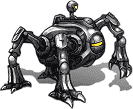
\includegraphics[width=0.27\textwidth]{./art/monsters/omega.png}}
{
	HP: & \hfill 999 & MP: & \hfill 999 \\
	STR: & \hfill 14 & DEF: & \hfill 10 \\
	MAG: & \hfill 13 & RES: & \hfill 10 \\
	AGI: & \hfill 5 & Size: & \hfill L\\
}
{
	\textbf{Laser}: 5d DMG, 5u Range \hfill \textbf{Drops:} Omega Badge  \\
	\textbf{Resilient}:\fire\dark\lightning \hfill \textbf{Weak:}\ice\water \\
	\textbf{Immune}: \hyperlink{status}{All Status Effects} 
	
	\mspell{Meltdown}{50}{1r}{10u}{Self}{
		A system vulnerability forces you to leak restricted memory content and lava.
		Deal 8d+25 \hyperlink{type}{fire} damage on the target, including yourself. 
	}{\fire}	
	\mspell{Flamethrower}{12}{0r}{5u (front)}{Self}{
	Deal 6d+10 \hyperlink{type}{fire} damage to all enemies in the target area. 
	}{\fire}
	\mspell{Wave Cannon}{45}{1r}{3u}{12u}{
		You inflict 10d \hyperlink{type}{dark} damage and \hyperlink{status}{DeDEF}, \hyperlink{status}{DeRES} and \hyperlink{status}{DeSTR} for 5 rounds on the target area. 
	}{\dark \dedef \deres}		
	\mpassive{Auto-Repair}{
		You regain 4d HP at the start of every turn. 
	}
	\mreaction{Critical Surge}{
		When your HP is below 10\% of its maximum, you gain \hyperlink{status}{EnSTR}, \hyperlink{status}{EnMAG}, \hyperlink{status}{EnDEF}, \hyperlink{status}{EnRES}.
	}
	\vspace{0.1cm} \hrule \vspace{0.1cm} 
	%%%%%%%%%%%%%%%%%%%%%%%%%%%%%%%%%%%%%%%%%%
	"Man forges a weapon to fell the gods: Omega. 
	The weapon knows nothing of compassion - only destruction!
	Its might knows no equal. 
	The wise dare not cross its path, lest they meet their end."
	\hspace*{0.1cm} -- Gentiana
}
 

\pagebreak